%!TEX root = ../thesis.tex
%*******************************************************************************
%****************************** Second Chapter *********************************
%*******************************************************************************

\chapter{Conclusion and Outlook}
\label{sec:out}

This work describes multiple measurements of the top quark pair production cross section in proton-proton collisions at a center of mass energy of $\sqrt{s}=13 \TeV$ with two leptons in the final state.
Three separate measuremnts are performed using data sets with an integrated luminosity of $\mathcal{L}_{\mathrm{int}}= 42 \pbinv$, $\mathcal{L}_{\mathrm{int}}= 2.2 \fbinv$ and $\mathcal{L}_{\mathrm{int}}= 35.9 \fbinv$.
The last of these three measurements, using data with the highest luminosity, is the main result of this work.
The measurements are performed with a binned maximum likelihod fit using observables of jet kinematics as templates. 
Systematic uncertainties are included as nuisance parameters.

In the full phase space the cross section for the three datasets mentioned previously is measured to be:

\begin{eqnarray*}
\sttbar & = & 778 \pm  54 ({\rm stat}) \pm 61 ({\rm syst}) \pm 76 ({\rm lumi}) \pb \hspace{0.2cm}  \mathrm{for} \; \;  \mathcal{L}_{\mathrm{int}}= 42 \pbinv, \\
\sttbar & = & 793 \pm  7 ({\rm stat}) \pm 27 ({\rm syst}) \pm 21 ({\rm lumi}) \pb  \hspace{0.2cm}  \mathrm{for} \;\; \mathcal{L}_{\mathrm{int}}= 2.2 \fbinv, \\
\mathrm{and} \; \; \sttbar & = & \resultxsecmain \hspace{0.2cm}  \mathrm{for} \;\; \mathcal{L}_{\mathrm{int}}= 35.9 \fbinv.
\end{eqnarray*} 

These results show a continously improved precision for the measurement of the \ttbar production cross section. The last (main) result being the most precise, with a total uncertainty of \uncertaintytotmain. 
For the main result the \ttbar cross section  is measured in the dilepton channel including events from the \emu, \mumu and \ee channel.
Before the extrapolation to the full phase space the \ttbar production cross section is also measured in the visible phase space, as defined by the requirements for the leptons ($\pt(\mathrm{lead}) > 25 \GeV$, $\pt(\mathrm{sublead}) > 20 \GeV$, $\mll > 20 \GeV$).
For the main result the \ttbar production cross section in the visible phase space is measured as:

\begin{eqnarray*}
\sttvis & = & \resultxsecvismain. 
\end{eqnarray*}


The main result for the \ttbar production cross section is used to extract the top quark pole mass with the xFitter framework \cite{Alekhin:2014irh}:

\begin{equation}
\mtp = 171.9 \pm 1.4 \mathrm{(exp+pdf+\as)} \pm 2.0 \mathrm{(scale)} \pm 0.2 \mathrm{(\mtMC)} GeV . 
\end{equation}

The precision of the extracted top quark pole mass is limited by the theory (scale) uncertainty, so the precision of the \ttbar production cross section used for the 
extraction does not significantly influence the precision. 

The main result for the measurement of the \ttbar production cross section is compared to previous results as well as theory predictions in Figure \ref{fig:sum}.
It agrees well with the theoretical predictions as well as with other measurements. Compared to previous measurements by both CMS
and ATLAS it is one of the most precise measurements of the \ttbar cross section at $\sqrt{s} = 13 \TeV$.

\begin{figure}[htbp!]
  \begin{center}
    \resizebox{0.65 \textwidth}{!}{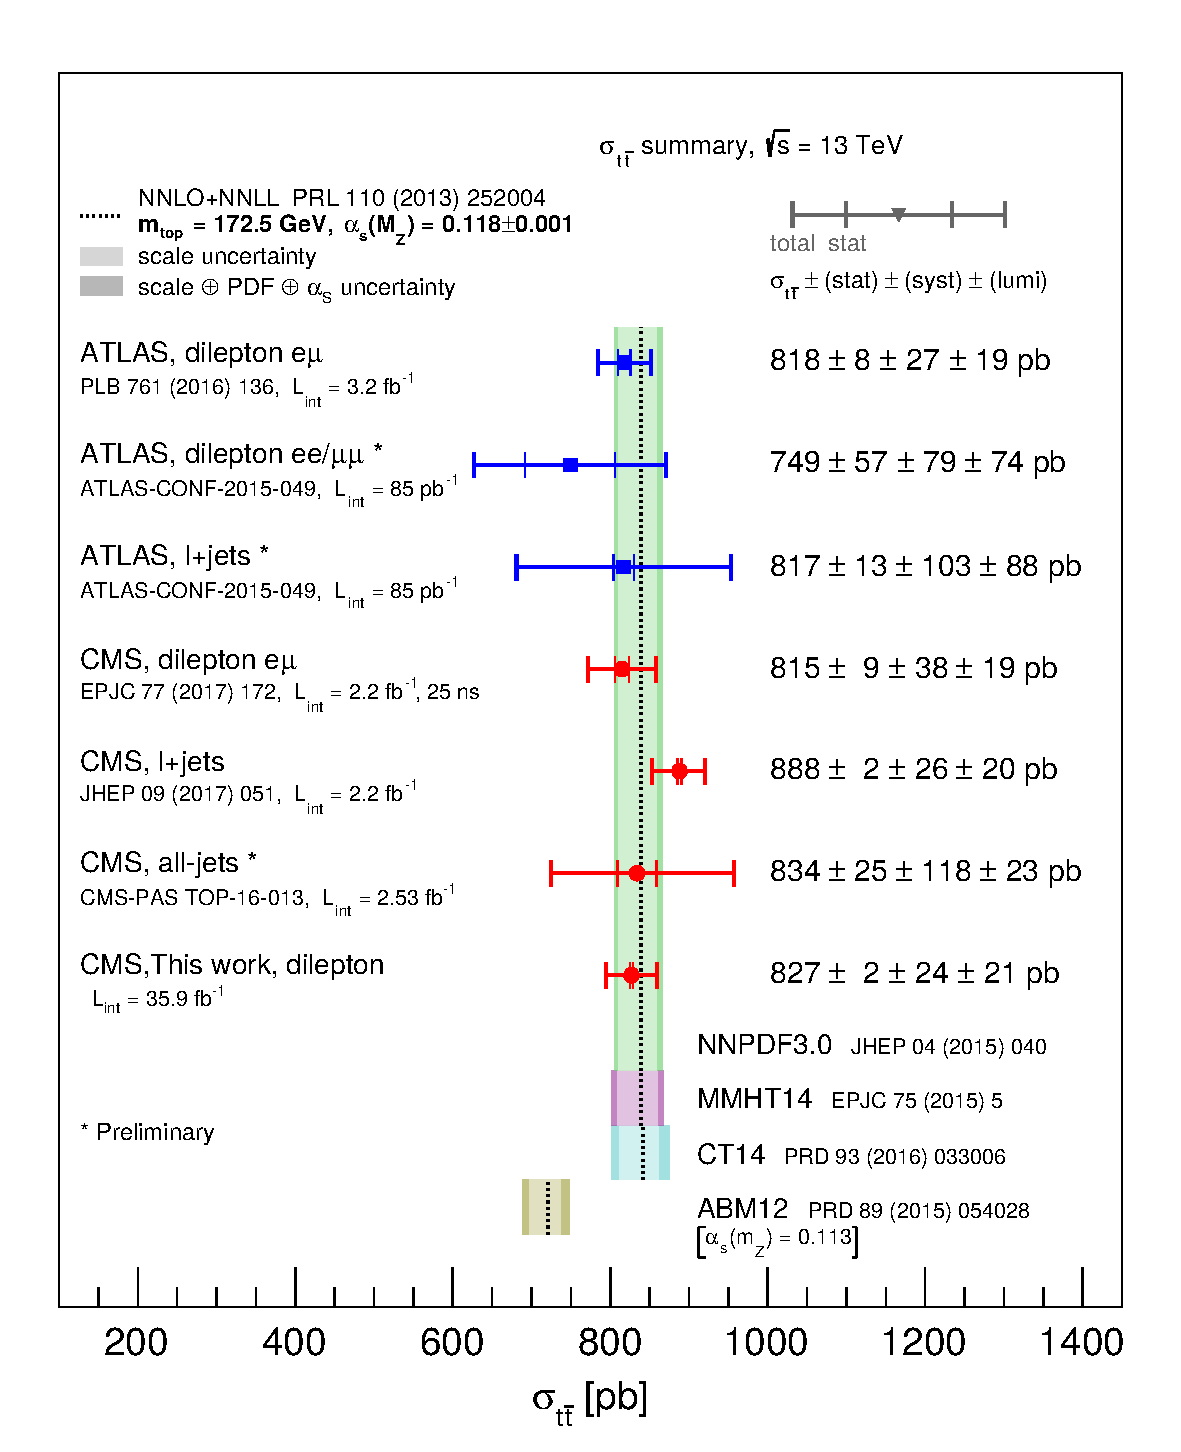
\includegraphics{Conclusion/Figures/tt_xsec_lhc13_Feb18}}   

\caption{Summary of measurements of the \ttbar production cross section at $\sqrt{s}=13 \TeV$ by the CMS and ATLAS collaboration.
The main result presented in this work is shown as well. All measurements are compared to theory predictions for different PDF sets.
Modified from \cite{Topsum}.
       \label{fig:sum}}
  \end{center}
\end{figure}

All measurements of the \ttbar cross section with different datasets and different experiments agree with the Standard Model prediction.
The measurements from different experiments have now reached comparable sensitivity to the theoretical prediction. Nevertheless, improving the exerimental sensitivity is still important.

The cross section measurement as presented here can be expanded to include a simultaneous fit of the cross section and the top quark mass.
This allows for a coherent treatment of the correlation of top quark mass and the \ttbar production cross section.
The measured \ttbar production cross section can be used to extract
further Standard Model parameters like the strong coupling, \as. These results are currently prepared for a paper publication, together with the cross section measurement presented in this work.

The precision of the \ttbar production cross section measurement could be improved by reducing systematic uncertainties.
Since the systematic uncertainty is dominated by the uncertainty on the lepton efficiencies, a precise determination of the lepton efficiencies would improve the precision of the \ttbar production cross section measurement.
Similar to the study of the trigger efficiency in this work, a lepton efficiency measurement tailored specifically for this purpose could reduce the relevant uncertainty.
With a large amount of data it might be possible to measure the lepton efficiency in \ttbar events, by using kinematically reconstructed top quarks. Using the tag-and-probe technique, a hadronically 
decaying top quark could be the 'tag', while a leptonically decaying top quark could be used as a 'probe'.

Another way to further improve the measurement would be a combination with the semi leptonic \ttbar decay channel. As demonstrated in this work, such a combination has the potential to significantly reduce the uncertainties.
If that study where to be extended to a proper measurement, special care would be needed for the definition of the visible phase space and the corresponding event selection. With a looser event selection the separation between
signal and background would become more challenging, as well as the determination of the contribution of background processes including fake leptons.

The measurement of the \ttbar production cross section presented in this work could be extended by fitting the cross section in bins of relevant kinematic observables.
These differential results could be more sensitive to physics phenomena beyond the SM.

Top quark physics are also a relevant topic for experiments beyond the LHC: At a linear electron-prositron collider the top quark mass could be measured with a precision below a $100 \MeV$ by using a scan
of the collision energy around the threshold for top quark pair production \cite{Seidel2013}. A circular proton-proton collider at a center of mass energy of $\sqrt{s}=100 \TeV$ would produce on the order
of $10^{12}$ top quarks, which would allow for precise measurements of previously inaccessible processes.

In conclusion, a lot of possibilities to further extend or improve the measurement remain, a even though a high precision for the measurement of the top quark pair production cross section has been achieved, as presented in this work, .

